\documentclass[../../main.tex]{subfiles}

\graphicspath{{\subfix{../../immagini/}}}

\begin{document}
    Negli esperimenti del capitolo \ref{sec:valutazioneClassificatori} tutti i risultati presentati, per quanto riguarda la model evaluation, sono stati ottenuti utilizzando una tecnica che prende il nome di convalida incrociata, o cross validation. Scopo di questo paragrafo è di presentare una breve introduzione a questa tecnica.

    La procedura di convalida incrociata può essere riassunta nei seguenti passaggi: 
    \begin{itemize}
        \item \textsc{passo 1}: il dataset viene suddiviso in $k$ sottoinsiemi, tutti di egual dimensione,
        \item \textsc{passo 2}: viene selezionato uno dei $k$ sottoinsiemi, questo verrà utilizzato come test set,
        \item \textsc{passo 3}: il modello viene addestrato sul training set composto dai $k-1$ sottoinsiemi rimasti,
        \item \textsc{passo 4}: le prestazioni del modello addestrato vengono valutate sul test set (tramite una o più metriche a scelta),
        \item \textsc{passo 5}: si ricomincia dal passo 2 selezionando un nuovo sottoinsieme $k$ ancora non utilizzato come test test. Il processo terminerà una volta che tutti i sottoinsiemi saranno stati utilizzati come test set in una iterazione. Saranno quindi necessarie un totale di $k$ iterazioni.
    \end{itemize}

    Al termine della procedura di convalida viene fornita una valutazione delle prestazioni del modello calcolando la media aritmetica dei valori delle metriche calcolati ad ogni iterazione.

    \begin{figure}[H]
        \centering
        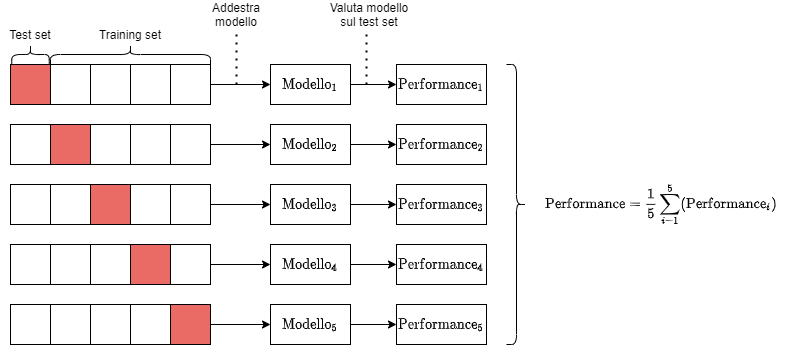
\includegraphics[width=\textwidth]{immagini/6_3/cross_validation.drawio.png}
        \caption{}
        \label{fig:crossvalidation}
    \end{figure}

    L'idea di questo approccio è di utilizzare ognuno degli esempi del dataset come elemento dell'insieme di test, e contemporaneamente di avere un training set ad ogni iterazione sufficiente ampio, in modo da eliminare un eventuale bias in negativo derivante da un training set troppo piccolo.

    La figura \ref{fig:crossvalidation} riassume il processo di model evaluation tramite convalida incrociata.
\end{document}